\documentclass{article}
\usepackage[utf8]{inputenc}
\usepackage[english]{babel}
 
\usepackage{hyperref}
\usepackage{graphicx}
\usepackage[margin=1.in]{geometry}

\hypersetup{
    colorlinks=true,
    linkcolor=blue,
    filecolor=magenta,      
    urlcolor=cyan,
}
 
\urlstyle{same}

\title{Competitive programming website - CodeArea
        CSP[203]: Software System Laboratory}
\date{\today}

\begin{document}

\maketitle

\begin{table}[h!]
    \begin{center}
    \scalebox{1.2}{
    \begin{tabular}{c c}
         Authors & email id \\
         \hline
         Girish Kumar  & 2016csb1040@iitrpr.ac.in \\
         Karan Seghal & 2016csb1080@iitrpr.ac.in\\
         Chirag Khurana & 2016csb1037@iitrpr.ac.in\\
         Arunaksha Talukdar & 2016csb1032@iitrpr.ac.in
    \end{tabular}
    }
    \end{center}
\end{table}

\vspace{2cm}

\begin{figure}[h!]
    \centering
    
\includegraphics[width=0.4\linewidth]{rpr_logo.jpg}
\end{figure}


\newpage


\section{Overview}
The main objective of this site is to provide students a competitive programming platform so students can compete with each other and can improve the competitive programming environment in the college. Through this website teachers will be able to create lab exams on competitive programming e.g. Data Structure.
The primary objective of the site is to reduce plagiarism from the internet while using other sites like Hackerrank, Codechef, to access these sites one need access to internet which lead to plagiarism. But the CodeArea site can be hosted on our servers, which can be accessed on the intranet.

\subsection{Technical Details}
We are using Postgres has our backend with Django, a python based web-framework. For frontend, we are using HTML5, CSS3 and few javascript libraries. The judge is also written in python.


% Girish %
\section{Judge}

\subsection{Introduction}
This is the important part of the CodeArea (competitive programming site name).
Main work of the judge is to execute user's codes and give them results of the execution e.g output for corresponding input or errors, compile time or run time errors. The judge take care of security and checks if the user program is not going to read or write other files on the server and executing other programs on the server.


\subsection{Supported languages}
In initial phase of the CodeArea we are supporting following programming languages:
\begin{enumerate}
    \item C
    \item C++14
    \item C++11
    \item JAVA 8
    \item Python 3.5
    \item Python 2.6
\end{enumerate}

\subsection{Facilities}
\vspace{0.3cm}
\subsubsection{Custom input-output}
To test the code we are providing custom input-output facility so user can test there code for corresponding input and output. Custom input-output will be implemented in the web-page using iframe.
\newpage
\subsubsection{Code Editor}
To make writing code easier, we are providing a code editor which can be implemented in the web-page using iframe. The editor provides basic functionalities of syntax highlighting, smart indenting, bracket completion, editor themes, fonts(small, medium, large).
All of these functionalities are powered by \href{https://ace.c9.io/}{ACE}, an open source library for code editor.
\begin{figure}[h!]
    \centering
    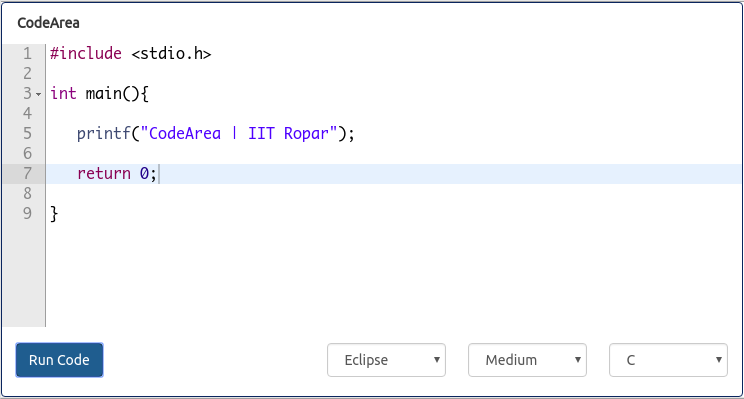
\includegraphics[width=0.8\linewidth]{sample_code_editor.png}
    \caption{ACE code editor}
    \label{fig:code_editor}
\end{figure}


\vspace{1.4cm}

\subsection{Submission}
On submission the language and the code is send to a python script which save the code to a temporary file with proper extension and we run the code on the server using os.system(command) and the program execution is killed if it takes more than the specified time. The output of the stdout and stderr is passed to a file and the content of the file is given to the user. Which contain errors in case of compile-time or run-time errors or output of program in case of successful completion of user program.
In case of submission against some test cases the content of the file is compared with right output for the problem.


% Karan %

\newpage

\section{Models}

\subsection{Introduction}
A model is the single, definitive source of information about one’s data. It contains the essential fields and behaviors of the data one is storing. Generally, each model maps to a single database table. The Models module manages the data, logic and rules of the database.


\subsection{Schema}
Apart from the User Model, mentioned in the Social Auth Module, the major entities of the application are, Problem, Contest, Participant, Submission, Tag and Post.
\begin{figure}[h!]
    \centering
    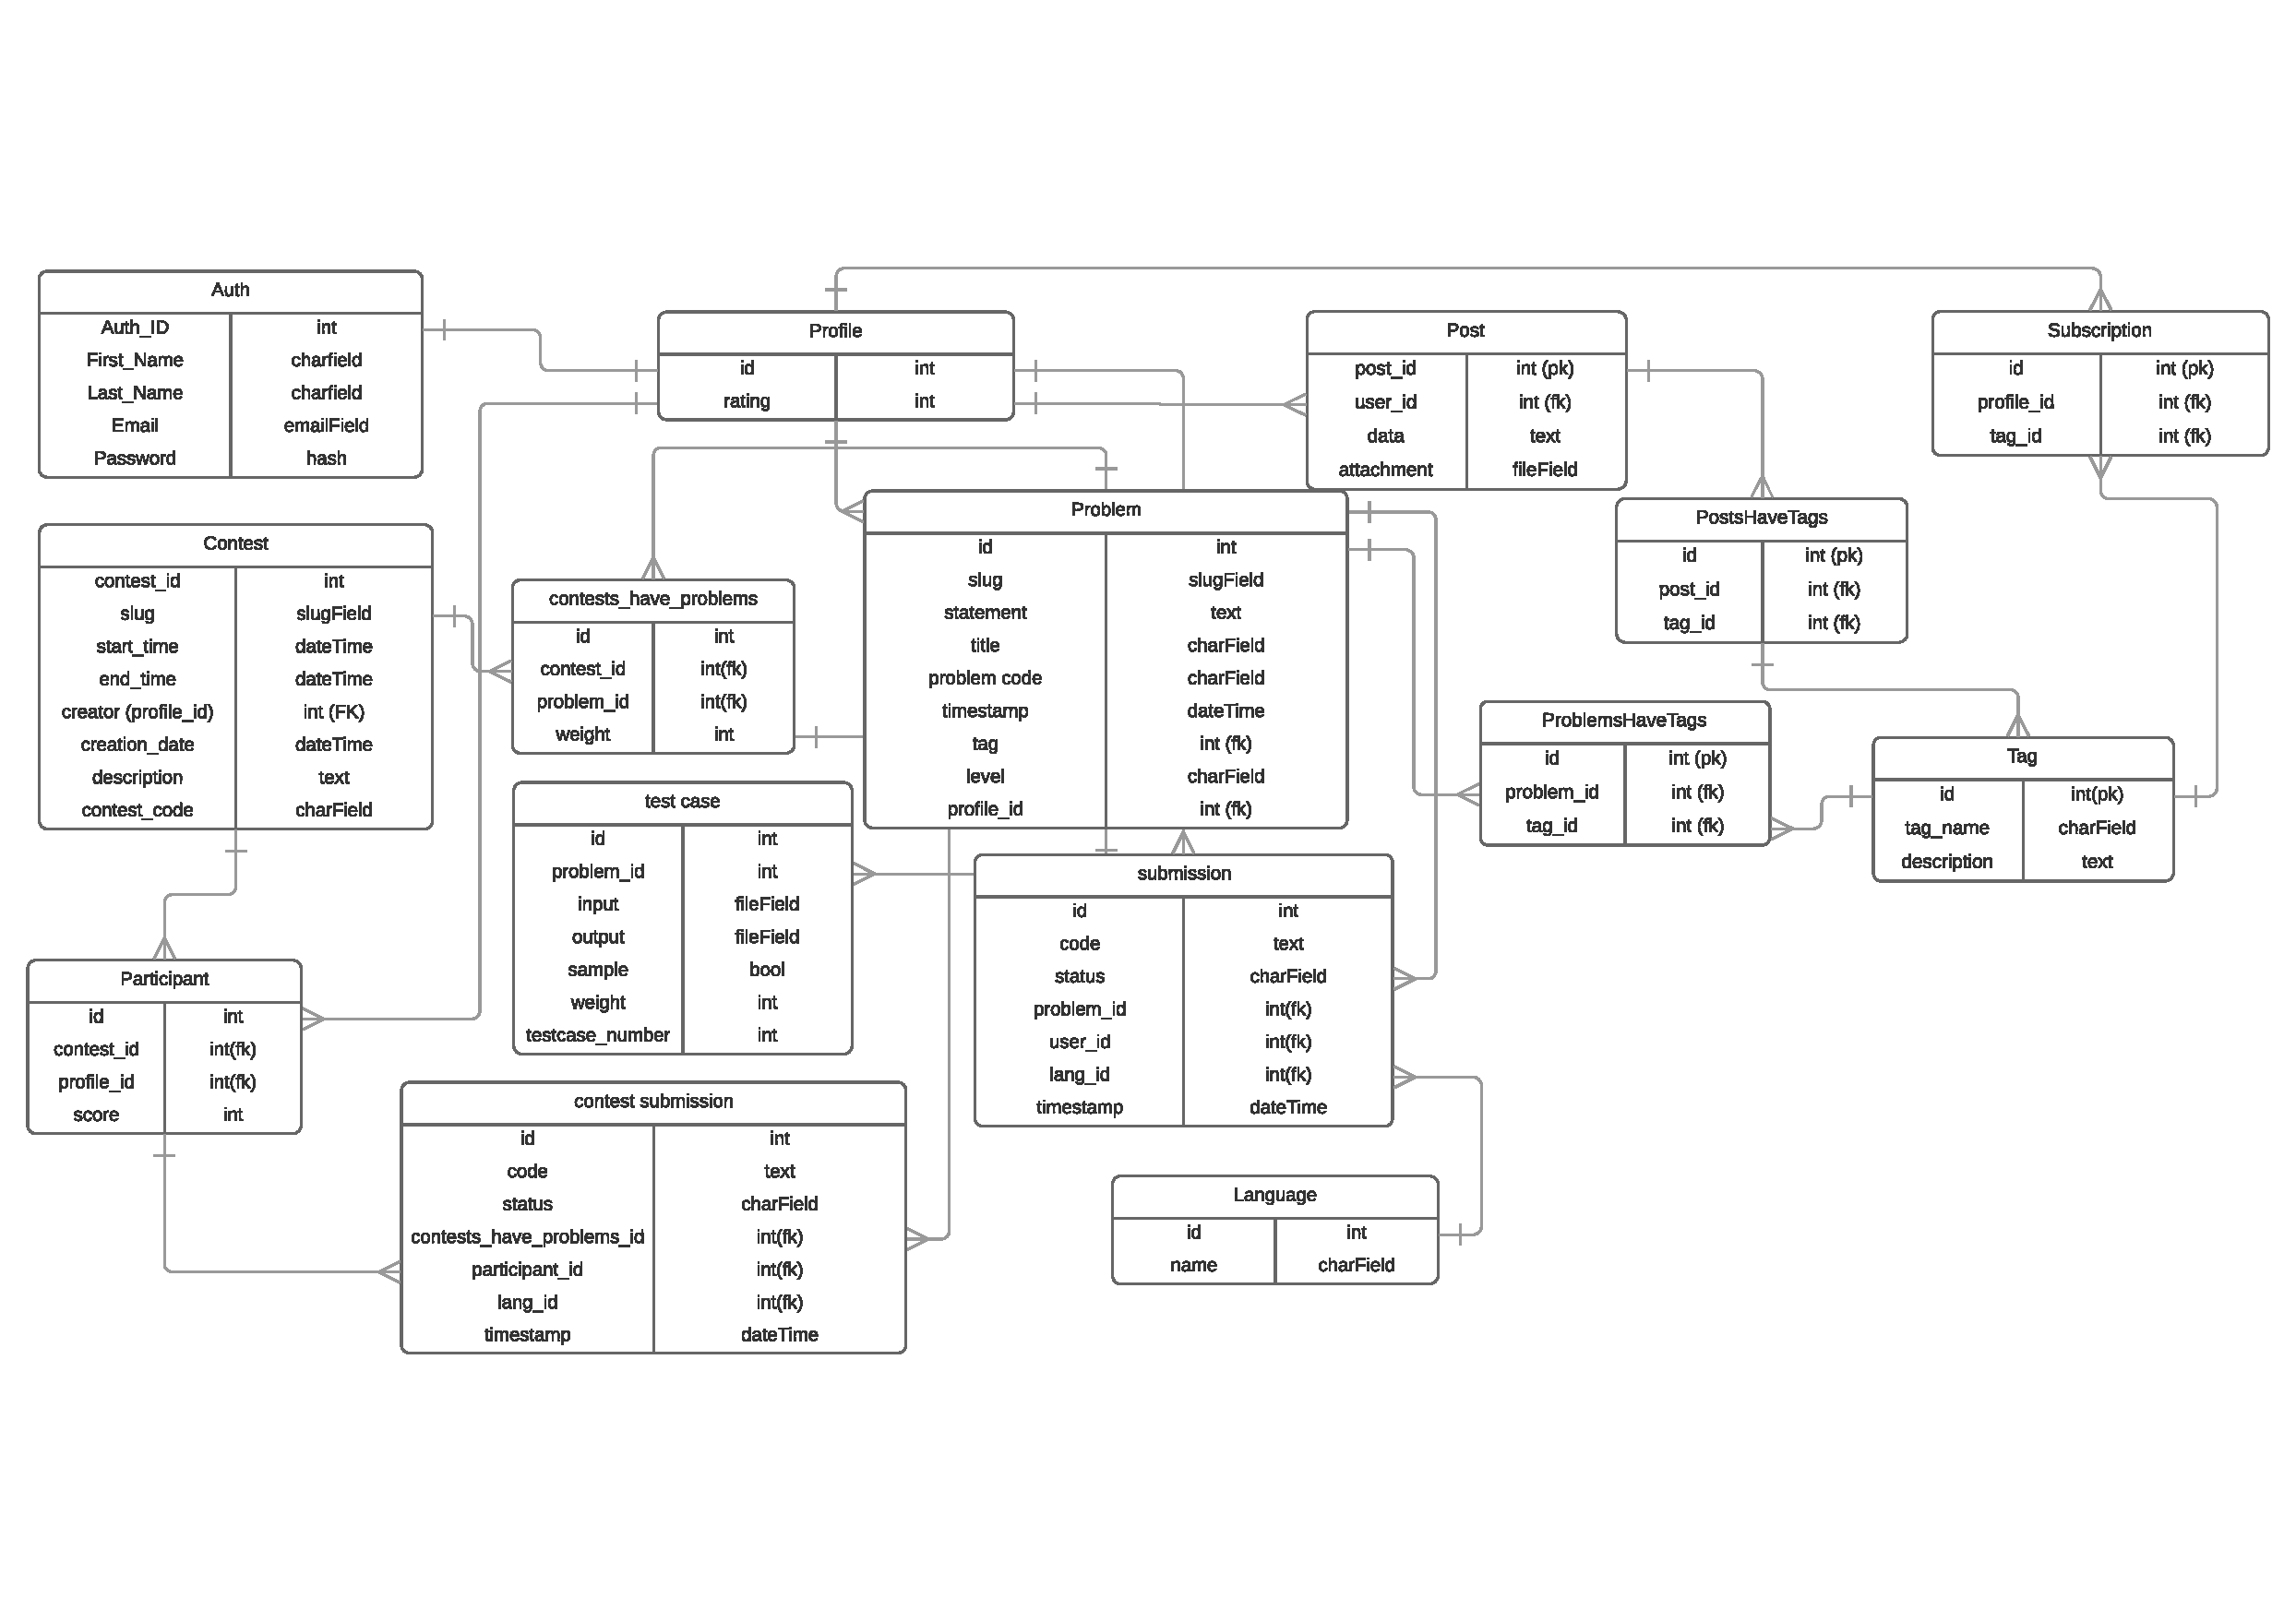
\includegraphics[width=\linewidth]{modules/schema.pdf}
    \caption{ER Diagram}
    \label{fig:schema}
\end{figure}

\vspace{1cm}

\subsubsection{Problem}
Consisting of a title, problem statement, level of difficulty, problem setter and test cases, the problem model represents a problem in the application. The model has a one-many relationship with Test Case, a many-one relationship with User and a many-many relationship with Contest. The model also contains problem code, which is a unique code given to the problem, as well as a slug field which is derived from the problem code. A slug field is used to store and generate valid URLs for dynamically created web pages. 

A \textit{pre\_save signal}, a signal (set of instructions) sent before the instance of a model is saved in the database, is used to generate a slug from the problem code.

\subsubsection{Test Case}
Consisting of an input file, an output file, test case number and weight, the Test Case Model represents a test case of a problem. The test case number attribute stores the value of the test case and the weight attribute representing the weight that specific test case has in the problem. There is a boolean attribute sample, which checks whether the test case is a sample test case.

The input and output files are stored in a folder named with the unique problem code, having names $<$test case number$>$.in and $<$test case number$>$.out, respectively.

\subsubsection{Contest}
Consisting of a title, description, starting time, ending time, and contest creator, the contest model represents a contest in the application. The model has a many-one relationship with User (creator of the contest), a many-many relationship with Problem and a many-many relationship with User (participants of the contest). The model also contains contest code, which is a unique code given to the problem, as well as a slug field, similar to the one in the Problem Model, which is derived from the problem code. 

\subsubsection{Contest Problem}
The many-many relationship between the Problem and Contest model is through the model Contest Problem, which represents a problem in the contest. Apart from foreign keys from both the models, it has a weight attribute representing the weight that specific problem has in the Contest.

\subsubsection{Participant}
The many-many relationship between the User and Contest model is through the model Participant, which represents a participant in a contest. Apart from foreign keys from both the models, it has a score attribute representing the total score of the user in the contest.

\subsubsection{Submission}
Consisting of a submitter, code, language, problem and status, the submission model represents a user submission. A user submission is sent to the Judge Module to get back the status of the submission. The current languages supported and status options are mentioned in the judge module.

\subsection{Future Plans}
Outside the contest environment, the application aims to extend its functionality by introducing two new models, Post and Tag, if time permits.

\subsubsection{Post}
Consisting of a title, description, optional attachment and creator, the post model represents a post. A post might be an article about some algorithm or some latest updates in the world of computer science. Various posts can be seen by a user on their homepage.

\subsubsection{Tag}
A tag is helpful in filtering out various posts and problems for a user. It has a many-many relationship with Post and Problem. Users can subscribe to specific tags to get updates on their feed.

% Anuraksha %

%----------------------------------------------------------
%                    Arunaksha Talukdar
%----------------------------------------------------------

\newpage

\section{Front-end of Code-Area}
The aim of the module is to develop the Frontend User Interaction module of Code-Area.

\subsection{Schema}
The website consist of hierarchical structure of linking of webpages as follow:
homepage , login page + about or Website Description , contestlist , contesthost , contest page , problem page , Rankboard.

\subsubsection{Homepage}
\begin{itemize}

\item Login region: Which verifies the user’s identification and grant’s further functionalities of the system.
\item About region: Describes a brief intro of the platform ,functionalities and suppotable code Formats.
\item Loginbox: Consist of userID, password entry box and Submit button handled by user authentication Module.

\end{itemize}

\subsubsection{Contestlist}
The ongoing contest at the moment or about to happen (With countdown time)

\subsubsection{Contesthost}
Raising a problem and Describing about it with the following functionalities supportable:
\begin{itemize}
\item Problem name 
\item Problem Description
\item Scores Description
\item Note box : regarding time limit , input limit
\item Save button: To Confirm and proceed.
\item Sample input , expected output with description
\end{itemize}

\subsubsection{Contestpage}
The main Contest page includes : Countdown timer till completion , Complete Problem Description ,Test cases with expected output. 

\subsubsection{Problem page}
\begin{itemize}
\item Short Problem descrition with Sample input ,expected output dialog box
\item Code input Submission Frame output managed by JUDGE module. With a management of
Code sumbimtted and rank in rankboard by DATABASE module.
\item Submit box: Link to Rankboard , and final submission of code.
\end{itemize}

\subsubsection{Rankboard}
\begin{itemize}
\item Shows rank of Coders (On basis of JUDGE module)
\item Resubmit Button: Option to revisit the problem and Modify it and submit without altering the previous Submit{No limit to Submissions }.
\end{itemize}
%----------------------------------------------------------

% TBD %
\newpage

\section{Forms}
The Forms Module manages the process of accepting input from the user, and then processing and responding to the input. Major functions performed by the module are as follows:
\begin{itemize}
	\item Preparing and restructuring data to make it ready for rendering
	\item Creating HTML forms for the data
	\item Receiving and processing submitted forms and data from the client
	\item Perform validation checks before saving the data to the database
\end{itemize}

\section{Views}
A view takes a Web request and returns a Web response. This response can be the HTML contents of a Web page, or a redirect, or a 404 error, or an XML document, or an image . . . or anything, really. The view itself contains whatever arbitrary logic is necessary to return that response. The View Module manages all the different views for different pages in the application, all views being their own submodules. All the CRUD operations operate through views. The major pages in the application are as follows:
\begin{itemize}
	\item Home Page
	\item Login Page
	\item Register Page
	\item Profile Page
	\item Problem Page
	\item Contest Page
	\item Contest Problem Page
	\item Submissions Page
\end{itemize}

\section{User Permissions}
Closely related to the Views Module, the User Permissions module manages all the user permissions of the app. User permissions include what all pages a user can view, what all files on the server can the user have access to, etc.

% Chirag %
\newpage

\section{Social Authentication}
\subsection{Introduction}
Social login is a form of single sign-on using existing information from a social networking service such as Facebook, Twitter or Google+, to sign into a third party website instead of creating a new login account specifically for that website.
Our mode of authentication is using the Google login.
\subsection{Features}
\begin{itemize}
	\item As almost every coder has Google account, he/she can easily sign in with Google without any signup.
	\item If we have to conduct a competition within the institute, we can put the filter which will allow only sign in with institute’s email-id.
	\item It saves database memory for storing credentials of the users.
	\item No need to send confirmation mail, and the email would be validated.

\end{itemize}
\subsection{Implementation}
We are using Django Social Auth library to implement this, it is an easy way to setup social authentication/authorization mechanism for Django projects. It provides user login using social websites credentials. It populates data from the social websites and creates new users.

We have a one-one relationship between a user and profile, extra application dependent information is stored in the profile model.


\section{Rich Text Integration}
\subsection{Introduction}
This module aims to integrate a rich text editor with the text field of a form, especially for problem statements and posts. This module can be integrated with either a markdown editor or a WYSIWYG (what you see is what you get) editor. Websites like hackerrank or stackoverflow use a markdown editor, since it is more customizable for people familiar with markdown.
\subsubsection{Markdown Editor}
Markdown is a lightweight markup language with plain text formatting syntax. It can be converted to HTML and many other formats. Markdown is often used to format readme files, for writing messages in online discussion forums, and to create rich text using a plain text editor.
\subsubsection{WYSIWYG Editor}
WYSIWYG implies a user interface that allows the user to view something very similar to the end result while the document is being created. In general, WYSIWYG implies the ability to directly manipulate the layout of a document without having to type or remember names of layout commands.
\subsection{Use}
The major use for this module to increase readability and writability in text fields like problem statement, contest description, post content, etc.
\subsection{Implementation}
There are several libraries compatible with Django for markdown editing (pagedown) as well as WYSIWYG (tinymce). This libraries allow addition of rich text editors in form fields.







\end{document}
